\documentclass[UTF8,11pt]{ctexart}
\usepackage[a4paper,margin=22mm]{geometry}
\usepackage{graphicx,enumitem,amssymb,tabularx}
\usepackage[normalem]{ulem}
\usepackage{xeCJKfntef}
\setlength{\parindent}{0pt}
\setlength{\parskip}{.6em}
\sloppy
\begin{document}
\section*{2020年12月英语四级真题(第2套)}
\subsection*{\textbf{Part I} \textbf{Writing} \textbf{( 30 minutes)}}


Directions: \textbf{\textit{For this part, you are allowed 80 minutes to write on the topic Changes in the Way of}} \textbf{\textit{Transportation. You should wr:ite at least 120 wonds but no more than 180 wa-ds.}}


\textbf{Part ll} \textbf{Listening Comprehension} \textbf{( 25 minutes)}


\subsection*{Section A}


\textbf{Directions: }\textbf{\textit{In this section, yo.u will hear three news reports. At the end of each news report, you w.ill hear}} \textbf{\textit{two or three questions. Both the news report and the questions will be spoken only once. After you hear a}} \textbf{\textit{question }}, \textbf{\textit{you m.ust choo-.w! the best answer from the four choices marked A) }}, \textbf{\textit{B) }}, \textbf{\textit{'C) and }}\textbf{D) . }\textbf{\textit{Then mark}} \textbf{\textit{the corresponding letter on Answer Sheet 1 with a single line through the centre.}}


\textbf{Questions 1 and 2 are based on the news report you have Just heanl.}


\textbf{1.}


\begin{itemize}[leftmargin=2em,itemsep=.2em,topsep=.4em]\item[A.] \textbf{He wanted to buy a home.}
\item[B.] \textbf{He suffered from a shock.}
\item[C.] \textbf{He lost a huge sum of money.}
\item[D.] \textbf{He did an unusual good deed.}
\end{itemize}

\textbf{2.}


\begin{itemize}[leftmargin=2em,itemsep=.2em,topsep=.4em]\item[A.] \textbf{Invite the waiter to a fancy dinner.}
\item[B.] \textbf{Tell her story to the }\textbf{\textit{Daily News.}}
\item[C.] \textbf{Give some money to the waiter.}
\item[D.] \textbf{Pay the waiter's school tuition.}
\end{itemize}

\textbf{Questions 3 and 4 are based on the news report yo11 have Just heanl}


\textbf{3.}


\begin{itemize}[leftmargin=2em,itemsep=.2em,topsep=.4em]\item[A.] \textbf{Whether or not to move •to the state's mainland.}
\item[B.] \textbf{How to keep the village from sinking into the sea.}
\item[C.] \textbf{Where to get the funds for rebuilding their village.}
\item[D.] \textbf{What to do about the rising level of the seawater.}
\end{itemize}

\textbf{4.}


\begin{itemize}[leftmargin=2em,itemsep=.2em,topsep=.4em]\item[A.] \textbf{It takes too long a time.}
\item[B.] \textbf{It costs too much money.}
\item[C.] \textbf{It has to wait for the state's fina} \textbf{l approval.}
\item[D.] \textbf{It faces strong opposition from many villagers.}
\end{itemize}

\textbf{Questions S to 7 are based on the news report you have Just heard.}


\textbf{5.}


\begin{itemize}[leftmargin=2em,itemsep=.2em,topsep=.4em]\item[A.] \textbf{To investigate whether people are grateful for help.}
\item[B.] \textbf{To see whether people hold doors open for strangers.}
\item[C.] \textbf{To explore ways of inducing gratitude in people.}
\item[D.] \textbf{To find out how people express gratitude.}
\end{itemize}

\textbf{6.}


\begin{itemize}[leftmargin=2em,itemsep=.2em,topsep=.4em]\item[A.] \textbf{They induced strangers to talk with them.}
\item[B.] \textbf{They helped 15 to 20 people in a bad mood.}
\item[C.] \textbf{They held doors open for people at various places.}
\item[D.] \textbf{They interviewed people who didn't say thank you.}
\end{itemize}

\textbf{7.}


\begin{itemize}[leftmargin=2em,itemsep=.2em,topsep=.4em]\item[A.] \textbf{People can be educated to be grateful.}
\item[B.] \textbf{Most people express gratitude for help.}
\item[C.] \textbf{Most people have bad days now and then.}
\item[D.] \textbf{People are ungrateful when in a bad mood.}
\end{itemize}

\subsection*{\textbf{Section B}}


\textbf{Directions: }\textbf{\textit{In this section, }}\textit{)OU }\textbf{\textit{will hear two long conversations. At the,end of each conver:sation, }}\textit{)OU }\textbf{\textit{will}} \textbf{\textit{hear four que.stions. Both the conver:sation and the questions will be spoken only once. After you hear a}} \textbf{\textit{question, you must choose the best answer from the four choices marked A), B), }}\textbf{C) }\textbf{\textit{and }}\textbf{D). }\textbf{\textit{Then mark}} \textbf{\textit{the ro"esponding letter on }}\textbf{Answer Sheet }\textbf{\textit{1 with a single line through the centre.}}


\textbf{Questions 8 to 11 are based on the conversation you have Just heard.}


\textbf{8.}


\begin{itemize}[leftmargin=2em,itemsep=.2em,topsep=.4em]\item[A.] \textbf{To order a solar panel installation.}
\item[B.] \textbf{To report a serious leak in his roof.} \textbf{.}
\item[C.] \textbf{To enquire about solar pai;iel installations.}
\item[D.] \textbf{To complain about the faulty: solar panels.}
\end{itemize}

\textbf{9.}


\begin{itemize}[leftmargin=2em,itemsep=.2em,topsep=.4em]\item[A.] \textbf{He plans to install solar pc1nels.}
\item[B.] \textbf{He owns a four-bedroom house.}
\item[C.] \textbf{He saves \$ 300 a year.}
\item[D.] \textbf{He has a large family.\_}
\end{itemize}

\textbf{10.}


\begin{itemize}[leftmargin=2em,itemsep=.2em,topsep=.4em]\item[A.] \textbf{Th.e service of the solar panel company.}
\item[B.] \textbf{The cost of a solar panel installation.}
\item[C.] \textbf{The maintenance of the solar panels.}
\item[D.] \textbf{The quality of the solar panels.}
\end{itemize}

. '


\noindent\begin{tabularx}{\linewidth}{@{}lXXXX@{}}\textbf{11.} & \textbf{A.} \textbf{One year and a half.} & \textbf{B.} \textbf{Less than four years.} & \textbf{C.} \textbf{Roughly six years.} & \textbf{D.} \textbf{About five years.}\\\end{tabularx}\par

\textbf{Questions 12 to 15 }are \textbf{based on the conversatim you have just heard.}


\textbf{12.}


\begin{itemize}[leftmargin=2em,itemsep=.2em,topsep=.4em]\item[A.] \textbf{At a travel agency.}
\item[B.] \textbf{At an Australian airport.}
\item[C.] \textbf{At an airline transfer service.}
\item[D.] \textbf{At a local transportation authority.}
\end{itemize}

\textbf{13.}


\begin{itemize}[leftmargin=2em,itemsep=.2em,topsep=.4em]\item[A.] \textbf{She would be able to visit more scenic spots.}
\item[B.] \textbf{She wanted to save as much money as possible.}
\item[C.] \textbf{She would like to have everything taken care of.}
\item[D.] \textbf{She wanted to spend more time with her family.}
\end{itemize}

\noindent\begin{tabularx}{\linewidth}{@{}lXXXX@{}}\textbf{14.} & \textbf{A.} \textbf{Four days.} & \textbf{B.} \textbf{Five days.} & \textbf{C.} \textbf{One week.} & \textbf{D.} \textbf{Two weeks.}\\\end{tabularx}\par

\textbf{15.}


\begin{itemize}[leftmargin=2em,itemsep=.2em,topsep=.4em]\item[A.] \textbf{Choosing some activities herself.}
\item[B.] \textbf{Spending Christmas with Australians.}
\item[C.] \textbf{Driving along the Great Ocean Road.} . .j • . .
\item[D.] \textbf{Leaming more about wine making.}
\end{itemize}

\subsection*{\textbf{Section C}}


\textbf{Directions: }\textbf{\textit{In this section }}\textbf{, }\textit{)OU }\textbf{\textit{w.ill hear thnee JXlssages. At the end of each passage }}\textbf{, }\textbf{\textit{you will hear three or}} \textbf{\textit{four questions. Both the passage and the questions will be spoken only once. After }}\textit{)'lU }\textbf{\textit{hear a question }}\textbf{, }\textit{)OU} \textbf{\textit{must choose the best answer from the four choices marked A }}\textbf{) , }\textbf{\textit{B }}\textbf{) , C ) }\textbf{\textit{and D }}\textbf{) . }\textbf{\textit{Then mark the}} \textbf{\textit{co"esponding letter on Answer }}\textbf{Sheet }\textbf{\textit{1 with a single line through the centre }}\textbf{.}


\textbf{Questions 16 to 18 are based on the p1m\&ge you have just heard.}


\noindent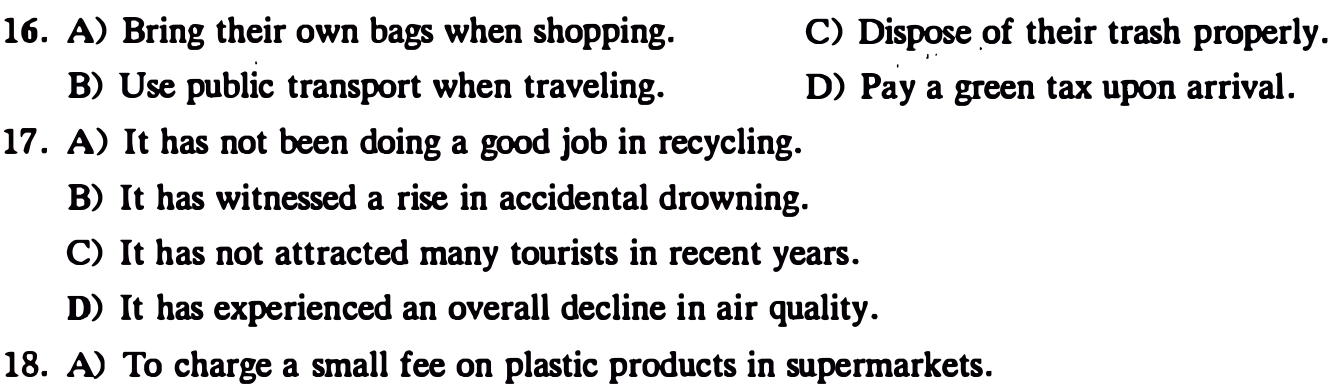
\includegraphics[width=\linewidth,height=.8\textheight,keepaspectratio]{2020-12-02.assets/char-002-line-022.png}\par

16.


\begin{itemize}[leftmargin=2em,itemsep=.2em,topsep=.4em]\item[A.] Bring their own bags when shopping.
\item[B.] Use public transport when traveling.
\item[C.] Dispose of their trash properly.
\item[D.] Pay a green tax upon arrival.
\end{itemize}

17.


\begin{itemize}[leftmargin=2em,itemsep=.2em,topsep=.4em]\item[A.] It has not been doing a good job in recycling.
\item[B.] It has witnessed a rise in accidental drowning.
\item[C.] It has not attracted many tourists in recent years.
\item[D.] It has experienced an overall decline in air quality.
\end{itemize}

18.


\begin{itemize}[leftmargin=2em,itemsep=.2em,topsep=.4em]\item[A.] To charge a small fee on plastic products in supermarkets.
\end{itemize}

\begin{itemize}[leftmargin=2em,itemsep=.2em,topsep=.4em]\item[B.] \textbf{To ban single-use plastic bags and straws on Bali Island.}
\item[C.] \textbf{• To promote the use of paper bags for shopping.}
\item[D.] \textbf{To impose a penalty on anyone caught littering.}
\end{itemize}

\textbf{Questions 19 to 21 are based on the passage you have just heard.}


\textbf{19.}


\begin{itemize}[leftmargin=2em,itemsep=.2em,topsep=.4em]\item[A.] \textbf{It gives birth to several babies at a time.}
\item[B.] \textbf{It is the least protected mammal species.}
\item[C.] \textbf{Its\textperiodcentered{}breeding grounds are now better preserved.}
\item[D.] \textbf{Its population is.now showing signs of increase.}
\end{itemize}

\noindent\begin{tabularx}{\linewidth}{@{}lXXXX@{}}\textbf{20.} & \textbf{A.} \textbf{Global warming.} & \textbf{B.} \textbf{Polluted seawaters.} & \textbf{C.} \textbf{Commercial hunting.} & \textbf{D.} \textbf{Decreasing birthrates.}\\\end{tabularx}\par

\noindent\begin{tabularx}{\linewidth}{@{}lXXXX@{}}\textbf{21.} & \textbf{A.} \textbf{To mate.} & \textbf{B.} \textbf{To look for food.} & \textbf{C.} \textbf{To escape hunters.} & \textbf{D.} \textbf{To seek breeding grounds.}\\\end{tabularx}\par

\textbf{Questions 22 to 25 are based on the passage you have just heard.}


\textbf{22.}


\begin{itemize}[leftmargin=2em,itemsep=.2em,topsep=.4em]\item[A.] \textbf{They prefer to drink low-fat milk.}
\item[B.] \textbf{They think milk is good for health.}
\item[C.] \textbf{They consume less milk these days.}
\item[D.] \textbf{They buy more milk than the British.}
\end{itemize}

\textbf{23.}


\begin{itemize}[leftmargin=2em,itemsep=.2em,topsep=.4em]\item[A.] \textbf{It is not as healthy as once thought.}
\item[B.] \textbf{It is not easy to stay fresh for long.}
\item[C.] \textbf{It benefits the elderly more.}
\item[D.] \textbf{It tends to make people fat.}
\end{itemize}

\textbf{24.}


\begin{itemize}[leftmargin=2em,itemsep=.2em,topsep=.4em]\item[A.] \textbf{They drink too many pints every dar\textperiodcentered{}.}
\item[B.] \textbf{They are sensitive to certain minerals.}
\item[C.] \textbf{They lack the necessary proteins to digest it.}
\item[D.] \textbf{They have eaten f,ood incompatible with milk.}
\end{itemize}

\textbf{25.}


\begin{itemize}[leftmargin=2em,itemsep=.2em,topsep=.4em]\item[A.] \textbf{It is easier for sick people to digest.}
\item[B.] It provides some necessary nutrients.
\item[C.] \textbf{It is healthier than other animal products.}
\item[D.] It supplies the body with enough calories.
\end{itemize}

\subsection*{\textbf{Part ]I[} \textbf{Reading Comprehension} \textbf{( 40 minutes)}}


\subsection*{\textbf{Section A}}


\textbf{Directions: }\textbf{\textit{In this section, there is a passage with ten blanks. You are required to select one word for each}} \textbf{\textit{blank from a list of choices given in a word bank following the passage. Read the passage through carefully}} \textbf{\textit{before making )VUr choices. Each choice in the bank is identified by a letter. Please mark the corresponding}} \textbf{\textit{letter for each item on }}\textbf{Answe,r }\textbf{\textit{Sheet }}\textbf{2\textperiodcentered{} }\textbf{\textit{with a single line through the centre. You may not }}ll.l? \textbf{\textit{any of the}} \textbf{\textit{words in the bank more than once.}}


\textbf{When my son completes a task, I can't help but praise him. It's only natural to give praise where}


\subsection*{\textbf{praise is due, right? But is there \textperiodcentered{}such a thing }as \textbf{too much praise?}}


\textbf{' praise as much as}


\subsection*{\textbf{According to psychologist Katherine Phillip, children don't-benefit from} \textbf{\uline{26}}}


\textbf{we'd like to think. " Parents' often praise, believing they are building their child's self-confidence.} \textbf{However, over-praising can have a} \textbf{\uline{27}} \textbf{effect," says Phillip. " When we use the same praise}


\noindent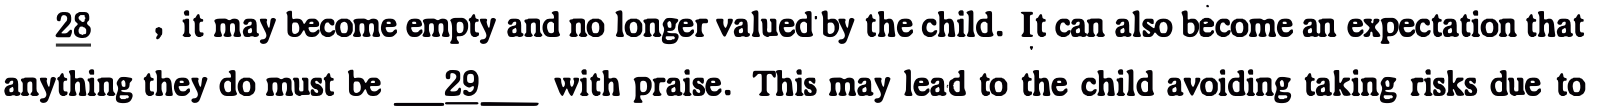
\includegraphics[width=\linewidth,height=.8\textheight,keepaspectratio]{2020-12-02.assets/char-003-line-022.png}\par

' .


\noindent
\includegraphics[width=\linewidth,height=.8\textheight,keepaspectratio]{2020-12-02.assets/char-003-line-024.png}\par

\textbf{Does this mean we should do away with all the praise? Phillip says no. "The key to healthy praise is to} \textbf{focus on the process rather than the} \textbf{\uline{31}} \textbf{. It is the recognition of a child's attempt, or the process in}


\noindent
\includegraphics[width=\linewidth,height=.8\textheight,keepaspectratio]{2020-12-02.assets/char-003-line-026.png}\par

\textbf{the risks needed to learn and grow. "}


\textbf{So how do we break the} \textbf{\uline{32}} \textbf{of praise we're all so accustomed to? Phillip says it's important to}


\noindent
\includegraphics[width=\linewidth,height=.8\textheight,keepaspectratio]{2020-12-02.assets/char-003-line-029.png}\par

\textbf{someone is. It's a form of personal approval. Process praise is acknowledgement of the efforts the person} \textbf{has just}----\textbf{35} \textbf{. Children who receive person praise are more likely to feel shame after losing," \textperiodcentered{}says} \textbf{Phillip.}


\begin{itemize}[leftmargin=2em,itemsep=.2em,topsep=.4em]\item[A.] \textbf{choose}
\item[B.] \textbf{constant}
\item[C.] \textbf{disappointing}
\item[D.] \textbf{distinguish}
\item[E.] \textbf{exhausting}
\item[F.] \textbf{experienced}
\item[G.] \textbf{negative}
\item[H.] \textbf{outcome}
\item[I.] \textbf{pattern}
\item[J.] \textbf{plural} \textbf{0) undertakeri}
\item[K.] \textbf{repeatedly}
\item[L.] \textbf{rewarded}
\item[M.] \textbf{separately}
\item[N.] \textbf{simply}
\end{itemize}

\subsection*{\textbf{Section B}}


\textbf{Directions: }\textbf{\textit{In this section, yo;u are going to read a passage with ten\textperiodcentered{} statements aitached to it. Each}} \textbf{\textit{statement contains information given in o.ne of the paragraphs. Identify the paragraph from which the}} \textbf{\textit{information is derived. You may choose a paragraph\textperiodcentered{} more than once. Each paragraph is marked with a}} \textbf{\textit{letter. Answer the questions by marking the cor.esponding }}\textbf{• }\textbf{\textit{letter on Answer Sheet 2.}}


\subsection*{\textbf{Poverty is a story about us, not them}}


A) \textbf{Too often still, we think we know what poverty looks like. 'It's the way we've been taught, the images} \textbf{we've been force-fed for decades. The chronically hoineless. The undocumented immigrant. The l} \textbf{urban poor, usually personified as a woman of color, the "welfare queen" politicians stil too often} \textbf{reference.}


B) \textbf{But as income inequality rises to record levels }in \textbf{the United States, even in the midst of a record} \textbf{economic expansion, those familiar images are outdated, hurtful, and counterproductive to focusing} \textbf{attention on solutions and building ladders of opportunity.}


C) \textbf{Today's faces of income inequality and lack of opportunity- look like all of us. It's Anna Landre, a} \textbf{disabled Georgetown University student fighting to keep health benefits that allow her the freedom to} \textbf{live her life. It's Tiffanie Standard, a counselor for young women of color in\textperiodcentered{}Philadelphia\textperiodcentered{}who want to} \textbf{be tech entrepreneurs-but who must work multiple jobs to\textperiodcentered{}stay afloat. It's Ken Outlaw, a welder in} \textbf{rural North Carolina whose dream of going back to school at a local community college was dashed by} \textbf{Hurricane Florence-just one of' the extreme weather events that have tipped the balance for struggling} \textbf{Americans across the nation.}


D) \textbf{If these are the central characters of our story about poverty, what layers of perceptions, myths, and} \textbf{realities must we unearth to find meaningful solutions and support? In pursuit of revealing this} \textbf{complicated reality, Mothering Justice, led by women of color, went last year to the\textperiodcentered{}state capital in} \textbf{Lansing, Michigan, to lobby on issues that affect working mothers. One of the Mothering Justice} \textbf{organizers went to the office of a state representative to talk about the lack of affordable childcare-} \textbf{the }\textbf{\textit{vestiges }}\raisebox{-0.331em}{
\includegraphics[height=1.395em]{2020-12-02.assets/char-004-001.png}}\allowbreak{}\raisebox{-0.334em}{
\includegraphics[height=1.416em]{2020-12-02.assets/char-004-002.png}}\allowbreak{}\raisebox{-0.334em}{
\includegraphics[height=1.416em]{2020-12-02.assets/char-004-003.png}}\allowbreak{}\textbf{ of a system that expected mothers to stay home with their children while their} \textbf{husbands worked. A legislative staffer dismissed the activist's concerns, telling her "my husband took} \textbf{care of that-I stayed home."}


E) \textbf{That comment, says Mothering Justice director Danielle Atkinson, '"was meant to shame" and relied} \textbf{on the familiar notion that a woman of color concerned about income inequality and programs that} \textbf{promote mobility must by definition be a-single\textperiodcentered{} morn, probably with multiple kids. In this case, the} \textbf{Mothering Justice activist happened to be married. And in \textperiodcentered{}most cases in the America of 2019, the} \textbf{images that come to mind when we hear the words poverty or income nequality fail miserably in}


\textbf{reflecting a complicated reality: poverty touches virtually all of us. The face of income inequality, for} \textbf{all but a very few of us, is the one we each see in the mirror.}


\begin{itemize}[leftmargin=2em,itemsep=.2em,topsep=.4em]\item[F.] \textbf{How many of us are poor in the U.S. ? It depends on who you ask. According to the Census Bureau,}
\end{itemize}

' \textbf{'} \textbf{38 million people in the U. S. are living below the official poverty thresholds. Taking into account} \textbf{economic need beyond that absolute measure, the Institute for Policy Studies found that 140 million} \textbf{people are poor or low-income. That's almost half the U.S. population.}


G) \textbf{Whatever the measure, within that massive group, poverty is extremely diverse. We know that some} \textbf{people are more affected than others, like children, the elderly, people with disabilities, and people} \textbf{of color.}


H) \textbf{But the fact that 4 in 10 ;Americans can't come up with \$.400 in an emergency is a commonly cited}


\noindent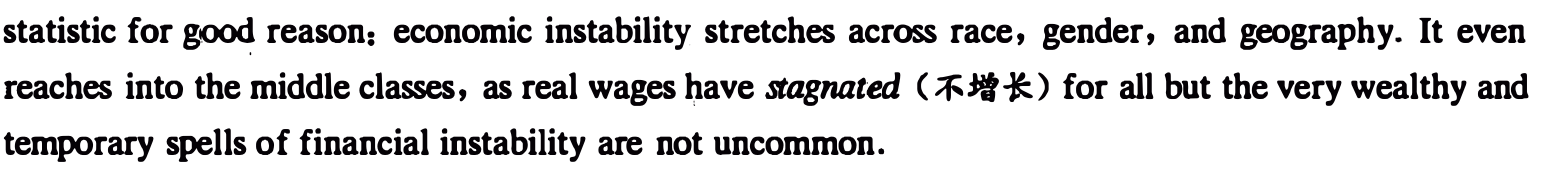
\includegraphics[width=\linewidth,height=.8\textheight,keepaspectratio]{2020-12-02.assets/char-005-line-005.png}\par

I) \textbf{Negative images remain of who is living in poverty as well as what is needed to move out of it. The big} \textbf{American myth is that yoµ can pull yourself up by your own efforts and change a bad situation into a} \textbf{good one. The reality is that finding opportunity without help from families, friends, schools, and} \textbf{community is virtually impossible. And the playing field is nothing close to level.}


J) \textbf{The Frame Works Institute, a research group that focuses on public framing of issues, has studied what}


\noindent
\includegraphics[width=\linewidth,height=.8\textheight,keepaspectratio]{2020-12-02.assets/char-005-line-008.png}\par

\textbf{and well being in life as a product 9f choice, willpower, and drive," says Nat Kendall-Taylor, CEO of} \textbf{Frame Works. "When we see people who are struggling," he says, those assumptions ''lead us to the} \textbf{perception that. people in poverty are lazy, they don't care, and they haven't made the right} \textbf{decisions. "}


K) \textbf{Does this sound familiar? Similar i<leas surround poverty in the U . S .. And these assumptions give a false} \textbf{picture of reality. "} \textbf{When people enter into that pattern of thinking," says Kendall-Taylor, "} \textbf{it's} \textbf{cognitively comfortable to make sense of issues of poverty in that way. It creates a kind of cognitive} \textbf{blindness-all of the factors external to a person's drive and choices that they've made become invisible }I \textbf{and fade from view. "}


L) \textbf{Those ex.temal factors include the difficulties accompanying low-wage work or structural} \textbf{discrimination based on race, gender, or ability. Assumptions get worse when people who are poor use} \textbf{government benefits to help them surviye. There is a great tension between "the poor" and those who} \textbf{are receiving what has become a dirty word: "welfare. "}


M) \textbf{According to the General Social Sqrvey, 71 percent of respondents believe the country is spending too} \textbf{\textperiodcentered{}little on "assistance to the. poor/' On the other hand, 22 percent think we are spending too little on} \textbf{"welfare": 37 percent -believe we are spending too much.}


N) \textbf{" Poverty has been interchangeable with people of color-specifically black women and black} \textbf{mothers," says Atkinson of Mothering Justice. It's true that black mothers are more affected by} \textbf{poverty than many other groups, yet they are. disproportionately the face of poverty. For example,} \textbf{Americans routinely overestimate the share of black recipients-of public assistance programs.}


\textbf{0) In reality, most people. will experience some form of financial hardship at some point in their lives.}


\textbf{Indeed, people tendto.dip in and out of poverty, perhaps due to unexpected obstacles like losing a job,}


\textbf{or when hours of a low-wage job fluctuate.} \textbf{P) Something each of us can do is to treat each other with the dignity and sympathy that is deserved and to} \textbf{understand deeply that the issue of poverty touches all of us.}


\textbf{36. One legislative staffer assumed that a woman of color who advocated affordable childcare must be a} \textbf{single mother.}


\textbf{37. People from different races, \_genders, and regions all suffer from a lack of financial security.}


\textbf{38. According to a survey, while the majority believe too little assistance is given to the poor, more than} \textbf{a third believe too much is spent on welfare.}


\textbf{39. A research group has found that Americans who are struggling are -thought to be lazy and to have made} \textbf{the wrong decisions.}


\textbf{40. Under the old system in America, a mother was supposed to stay home and take care of her children.}


\textbf{41. It was found that nearly 50\% of Americans are poor or receive low pay.}


\textbf{42. Americans usually overestimate the number of blacks receiving welfare benefits.}


\textbf{43. It is impossible for Americans to lift themselves out of poverty entirely on their own.}


\textbf{44. Nowadays, it seems none of us can get away from income inequality.}


\textbf{45. Assumptions about poor people become even more negative when-they live on welfare.}


\subsection*{\textbf{Section C}}


\noindent
\includegraphics[width=\linewidth,height=.8\textheight,keepaspectratio]{2020-12-02.assets/char-006-line-012.png}\par

\textbf{\textit{stltements. For each of them there are foo.r choices marked A), B), }}\textbf{C) }\textbf{\textit{and }}\textbf{D). }\textbf{\textit{You should decide on the}} \textbf{\textit{best choice and mark the corresponding letter on Answer Sheet 2 with a single line through the centre.}}


\subsection*{\textbf{Passage One}}


\textbf{Questions 46 to SO are based on the following passage.}


\textbf{Boredom has, paradoxically, become quite interesting to academics lately. In early May, London's} \textbf{Boring Conference celebrated seven years of delighting in dullness. At this event, people flocked to talks}


\subsection*{\textbf{about weather, traffic jams, and vending-machine sounds, among other sleep-inducing topics.}}


\textbf{What, exactly, is everybody studying? One widely accepted psychological definition of boredom is} \textbf{"the distasteful experience of wanting, but being unable, to engage in satisfying activity." But how can} \textbf{you quantify a person's boredom level and compare it with someone else's? In 1986, psychologists}


\noindent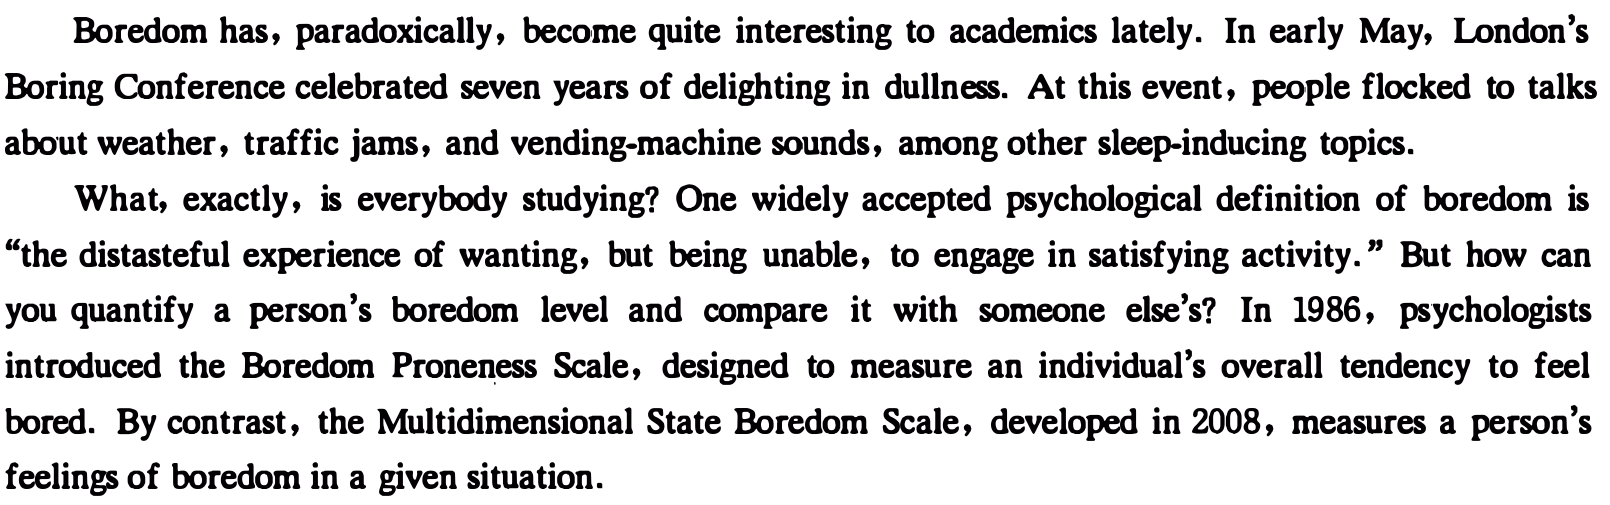
\includegraphics[width=\linewidth,height=.8\textheight,keepaspectratio]{2020-12-02.assets/char-006-line-019.png}\par

\textbf{bored. By contrast, the Multidimensional State Boredom Scale, developed in 2008, measures a person's} \textbf{feelings of boredom in a given situation.}


\textbf{Boredom has been linked to behavior issues including inattentive driving, mindless snac;:king, excessive} \textbf{drinking, and addictive gambling. In fact, many of us would choose pain over boredom. One team of} \textbf{psychologists discovered that two-thirds of men and a quarter of women would rather self-administer} \textbf{electric sbocks than sit alone with their thoughts for 15 minutes. R\_esearching this phenomenon, another} \textbf{team asked volunteers to watch boring, sad, or neutral films, during which they could self-administer} \textbf{electric shocks. The bored volunteers shocked • themselves more and harder than the sad or neutral} \textbf{ones did.}


\textbf{But boredom isn't all bad. By encouraging self-reflection and daydreaming, it can spur creativity. An} \textbf{early study gave participants abundant time to complete problem-solving and word-association exercises.} \textbf{Once all the obvious answers were exhausted, participants gave more and more inventive answers to}


\textbf{combat boredom. A British study took these findings one step further, asking subjects to complete a} \textbf{creative challenge (coming up with a list of alternative uses for a household item). One group of subjects} \textbf{did a boring activity first, while the others went straight to the creative task. Those whose boredom pumps} \textbf{had been primed were more productive.}


\textbf{In our always-connected world, boredom may be a hard-to-define state, but it is a fertile one. Watch} \textbf{paint dry or water boil, or at least put away your smartphone for a while, and you might unlock your next} \textbf{big idea.}


\textbf{46. When are people likely to experience boredom, according to an accepted psychological definition?}


\begin{itemize}[leftmargin=2em,itemsep=.2em,topsep=.4em]\item[A.] \textbf{When they don't have the chance to do what they want.}
\item[B.] \textbf{When they don't enjoy the materials they are studying.}
\item[C.] \textbf{When they experience something unpleasant ..}
\item[D.] \textbf{When they engage in some routine activities.}
\end{itemize}

\textbf{47. What does the author say boredom can lead to?}


\begin{itemize}[leftmargin=2em,itemsep=.2em,topsep=.4em]\item[A.] \textbf{Determination.}
\item[B.] \textbf{Concentration.}
\item[C.] \textbf{Mental deterioration.}
\item[D.] \textbf{Harmful conduct.}
\end{itemize}

\textbf{48. What is the finding of one team of psychologists in their experiment?}


\begin{itemize}[leftmargin=2em,itemsep=.2em,topsep=.4em]\item[A.] \textbf{Volunteers prefer watching a boring movie to sitting alone deliberating.}
\item[B.] \textbf{Many volunteers choose to hurt themselves rather than endure boredom.}
\item[C.] \textbf{Male volunteers are more immune to the effects of boredom than females.}
\item[D.] \textbf{Many volunteers are unable to resist boredom longer than fifteen minutes.}
\end{itemize}

\textbf{49. Why does the author say boredom isn't all bad?}


\begin{itemize}[leftmargin=2em,itemsep=.2em,topsep=.4em]\item[A.] \textbf{It stimulates memorization.}
\item[B.] \textbf{It allows time for relaxation.}
\item[C.] \textbf{It may promote creative thinking.}
\item[D.] \textbf{It may facilitate independent learning.}
\end{itemize}

\textbf{50. What does the author suggest one do when faced with a challenging problem?}


\begin{itemize}[leftmargin=2em,itemsep=.2em,topsep=.4em]\item[A.] \textbf{Stop idling and think big.}
\item[B.] \textbf{Unlock one's smartphone.}
\item[C.] \textbf{Look around oneself for stimulation.}
\item[D.] \textbf{Allow oneself some time to be bored.}
\end{itemize}

\subsection*{\textbf{Passage Two}}


\textbf{Questions 51 to 55 are based on the following pas.g1ge.}


\textbf{Forests in countries like Brazil and the Congo get a lot of attention\textperiodcentered{} from environmentalists, and it is} \textbf{easy to see why. South America and sub-Saharan Africa are experiencing deforestation on an enormous} \textbf{scale: every year almost 5 million hectares are lost. But forests are also changing in rich Western} \textbf{countries. They are growing larger, both in the sense that they occupy more land and that the trees in}


\noindent
\includegraphics[width=\linewidth,height=.8\textheight,keepaspectratio]{2020-12-02.assets/char-007-line-015.png}\par

\textbf{Forests are spreading in almost all Western countries, with the fastest growth in places that} \textbf{historically had rather few trees. In 1990 28\% of Spain was forested; now the proportion is 37\%. In both} \textbf{Greece and Italy, the growth was from 26\% to 32\% over the same period. Forests are gradually taking} \textbf{more land in America and Australia. Perhaps most astonishing is the trend in Ireland. Roughly 1\% of that} \textbf{country was forested when it became independent in 1922. Now forests cover 11 \% of the land, and the} \textbf{government wants to push the proportion to 18\% by the 2040s.}


\textbf{Two things are fertilising this \textperiodcentered{}growth. The first is the abandonment of farmland, especially in high,} \textbf{dry places where nothing grows terribly well. When farmers give up trying to earn a living from farming} \textbf{or herding, trees simply move in; The second is government policy and subsidy. Throughout history,}


\textbf{governments have protected and promoted forests for diverse reasons, ranging from the need for wooden} \textbf{warships to a desire to promote suburban house-building. Nowadays forests are increasingly welcome} \textbf{because they suck in carbon pollution from the air. The justifications change; the desire for more trees} \textbf{remains constant.}


\textbf{The greening of the West does not delight everyone. Farmers complain that land is being taken out of} \textbf{use by generously subsidised tree plantations. Parts of Spain and Portugal suffer from terrible forest fires.} \textbf{Others simply dislike the appearance of forests planted in neat rows. They will have to get used to the} \textbf{trees, however. The growth of Western forests seems almost as unstoppable as deforestation elsewhere.}


\textbf{51. What is catching environmentalists' attention nowadays?}


\begin{itemize}[leftmargin=2em,itemsep=.2em,topsep=.4em]\item[A.] \textbf{Rich countries are stripping poor ones of their resources.}
\item[B.] \textbf{Forests are fast shrinking in many developing countries.}
\item[C.] \textbf{Forests are eating away the fertile farmland worldwide.}
\item[D.] \textbf{Rich countries are doing little to address deforestation.}
\end{itemize}

\textbf{52. Which countries have the fastest forest growth?}


\begin{itemize}[leftmargin=2em,itemsep=.2em,topsep=.4em]\item[A.] \textbf{Those that have newly achieved independence.}
\item[B.] \textbf{Those that have the greatest demand for timber.}
\item[C.] \textbf{Those that used to have the lowest forest coverage.}
\item[D.] \textbf{Those that provide enormous government subsidies.}
\end{itemize}

\textbf{53. What has encouraged forest growth historically?}


\begin{itemize}[leftmargin=2em,itemsep=.2em,topsep=.4em]\item[A.] \textbf{The government's advocacy.}
\item[B.] \textbf{The use of wood for fuel.}
\item[C.] \textbf{The favourable climate.}
\item[D.] \textbf{The green movement.}
\end{itemize}

\textbf{54. What accounts for our increasing desire for forests?}


\begin{itemize}[leftmargin=2em,itemsep=.2em,topsep=.4em]\item[A.] \textbf{Their unique scenic beauty.}
\item[B.] \textbf{Their use as fruit plantations.}
\item[C.] \textbf{Their capability of improving air quality.}
\item[D.] Their stable supply of building materials.
\end{itemize}

\textbf{55. What does the author conclude about the prospects of forestation?}


\begin{itemize}[leftmargin=2em,itemsep=.2em,topsep=.4em]\item[A.] \textbf{Deserts in sub-Saharan Africa will diminish gradually.}
\item[B.] \textbf{It will play a more and more important role in people's lives.}
\item[C.] \textbf{Forest destruction in the developing world will quickly slow down.}
\item[D.] \textbf{Developed and developing countries are moving in opposite directions.}
\end{itemize}

\subsection*{\textbf{Part N} \textbf{Translation} \textbf{( 30 minutes)}}


\textbf{Directions: }\textbf{\textit{For this pari, ,vu are allowed 80 minutes to translate a passage from Chinese into E:nglish. You}} \textbf{\textit{should write ,our answer on Answer Sheet 2.}}


\noindent
\includegraphics[width=\linewidth,height=.8\textheight,keepaspectratio]{2020-12-02.assets/char-008-line-014.png}\par
\end{document}